\documentclass[12pt]{article}
\usepackage{amsmath,amsfonts}
\usepackage[cm]{fullpage}
\usepackage{graphicx}

\pagenumbering{gobble}

\title{\vspace{-24pt}March Monthly Problem Set Solutions}
\author{\vspace{-24pt}}
\date{\vspace{-24pt}}


\begin{document} \maketitle \pagestyle{empty}

\begin{enumerate}

\item % Easy, Dutch BxMO Selection Test 2016
%For a positive integer that is not a power of 2, define $t(n)$ as the greatest odd divisor of $n$ and $r(n)$ as the smallest odd divisor of $n$ greater than 1. Determine all positive integers $n$ which are not powers of 2 and satisfy
%	\[ n = 3t(n)+5r(n).\]
Let $n = 2^{k(n)} \cdot t(n)$. Note that $r(n)$ divides $t(n)$, and so we can
write $t(n) = s(n) r(n)$ for some natural number $s(n)$. The condition $n =
3t(n) + 5r(n)$ is then equivalent to
\[
    2^{k(n)} s(n) r(n) = 3 s(n) r(n) + 5r(n),
\]
or, equivalently,
\[
    2^{k(n)} s(n) = 3s(n) + 5.
\]

If $k(n) \leq 1$, then we have that
\[
    2^{k(n)} s(n) \leq 2s(n) < 3s(n) + 5
\]
since $s(n)$ is positive, and so we have no solutions in this case.

If $k(n) = 2$, then the equation is equivalent to $4s(n) = 3s(n) + 5$, which
gives us that $s(n) = 5$. Since $s(n) = 5$ is an odd divisor of $n$, we then
require that $r(n) \leq 5$, and so $r(n) \in \{3, 5\}$. Recalling that
\[
    n = 2^{k(n)} s(n) r(n) = 2^2 \cdot 5 \cdot r(n) = 20 r(n),
\]
we thus find the solutions $n = 60$ and $n = 100$.

Finally, if $k(n) \geq 3$, then we have that
\[
    3s(n) + 5 = 2^{k(n)} s(n) \geq 8 s(n) = 3s(n) + 5s(n) \geq 3s(n) + 5,
\]
and, since equality occurs, we must have that $k(n) = 3$ and $s(n) = 1$.
Recalling that
\[
    n = 2^{k(n)} s(n) r(n) = 2^3 \cdot 1 \cdot r(n) = 8r(n),
\]
and noting that $r(n)$ is a prime number, we thus find the family of solutions
$n = 8p$ where $p$ is a prime number.

All solutions are thus given by $n = 60$, $n = 100$, and $n = 8p$ where $p$ is
an odd prime number.


\item % PP-2005-3
%$ABCD$ is a square. At $B$, another square $BEFG$ is drawn so that $\angle ABE$ is obtuse. Prove that the median through $B$ of triangle $BCG$ is perpendicular to $AE$.
Let $M$ be the midpoint of $CG$. Let $\Gamma_1$ be the circle with centre $A$
and radius $AB$, and $\Gamma_2$ be the circle with centre $E$ and radius $EB$.
Since $AE$ is the line between the entre of these two circles, it is enough to
show that $MB$ is the radical axis of $\Gamma_1$ and $\Gamma_2$. The point $B$
lies on both circles, so we just need to show that $M$ has equal power with
respect to each circle. Thus we wish to show that $MA^2 - AB^2 = ME^2 - EB^2$.

By the cosine law in triangles $\triangle MAB$ and $\triangle MEB$, we have that
\[
    MA^2 - AB^2 = MB^2 - 2 AB \cdot MB \cos(\angle MBA),
\]
and
\[
    ME^2 - EB^2 = MB^2 - 2 EB \cdot MB \cos(\angle EBM).
\]

It is thus enough to show that $AB \cos(\angle MBA) = EB \cos(\angle EBM)$. Now
note that $\cos(\angle MBA) = \cos(90^\circ + \angle MBC) = -\sin(\angle MBC)$,
and, similarly, $\cos(\angle EBM) = -\sin(\angle GBM)$. Thus we wish to show
that $AB \sin(\angle MBC) = EB \sin(\angle GBM)$. Since $AB = BC$, and $EB =
BG$, this is equivalent to $BC \sin(\angle MBC) = BG \sin(\angle GBM)$

The sine law in triangles $\triangle BGM$ and $\triangle BMC$ gives us that $BC
\sin(\angle MBC) = MC \sin(\angle CMB)$, and $BG \sin(\angle GBM) = GM
\sin(\angle BMG)$. Since $GM = MC$ and $\sin(\angle CMB) = \sin(\angle BMG)$,
the result follows.

\begin{figure}[!ht]
\centering
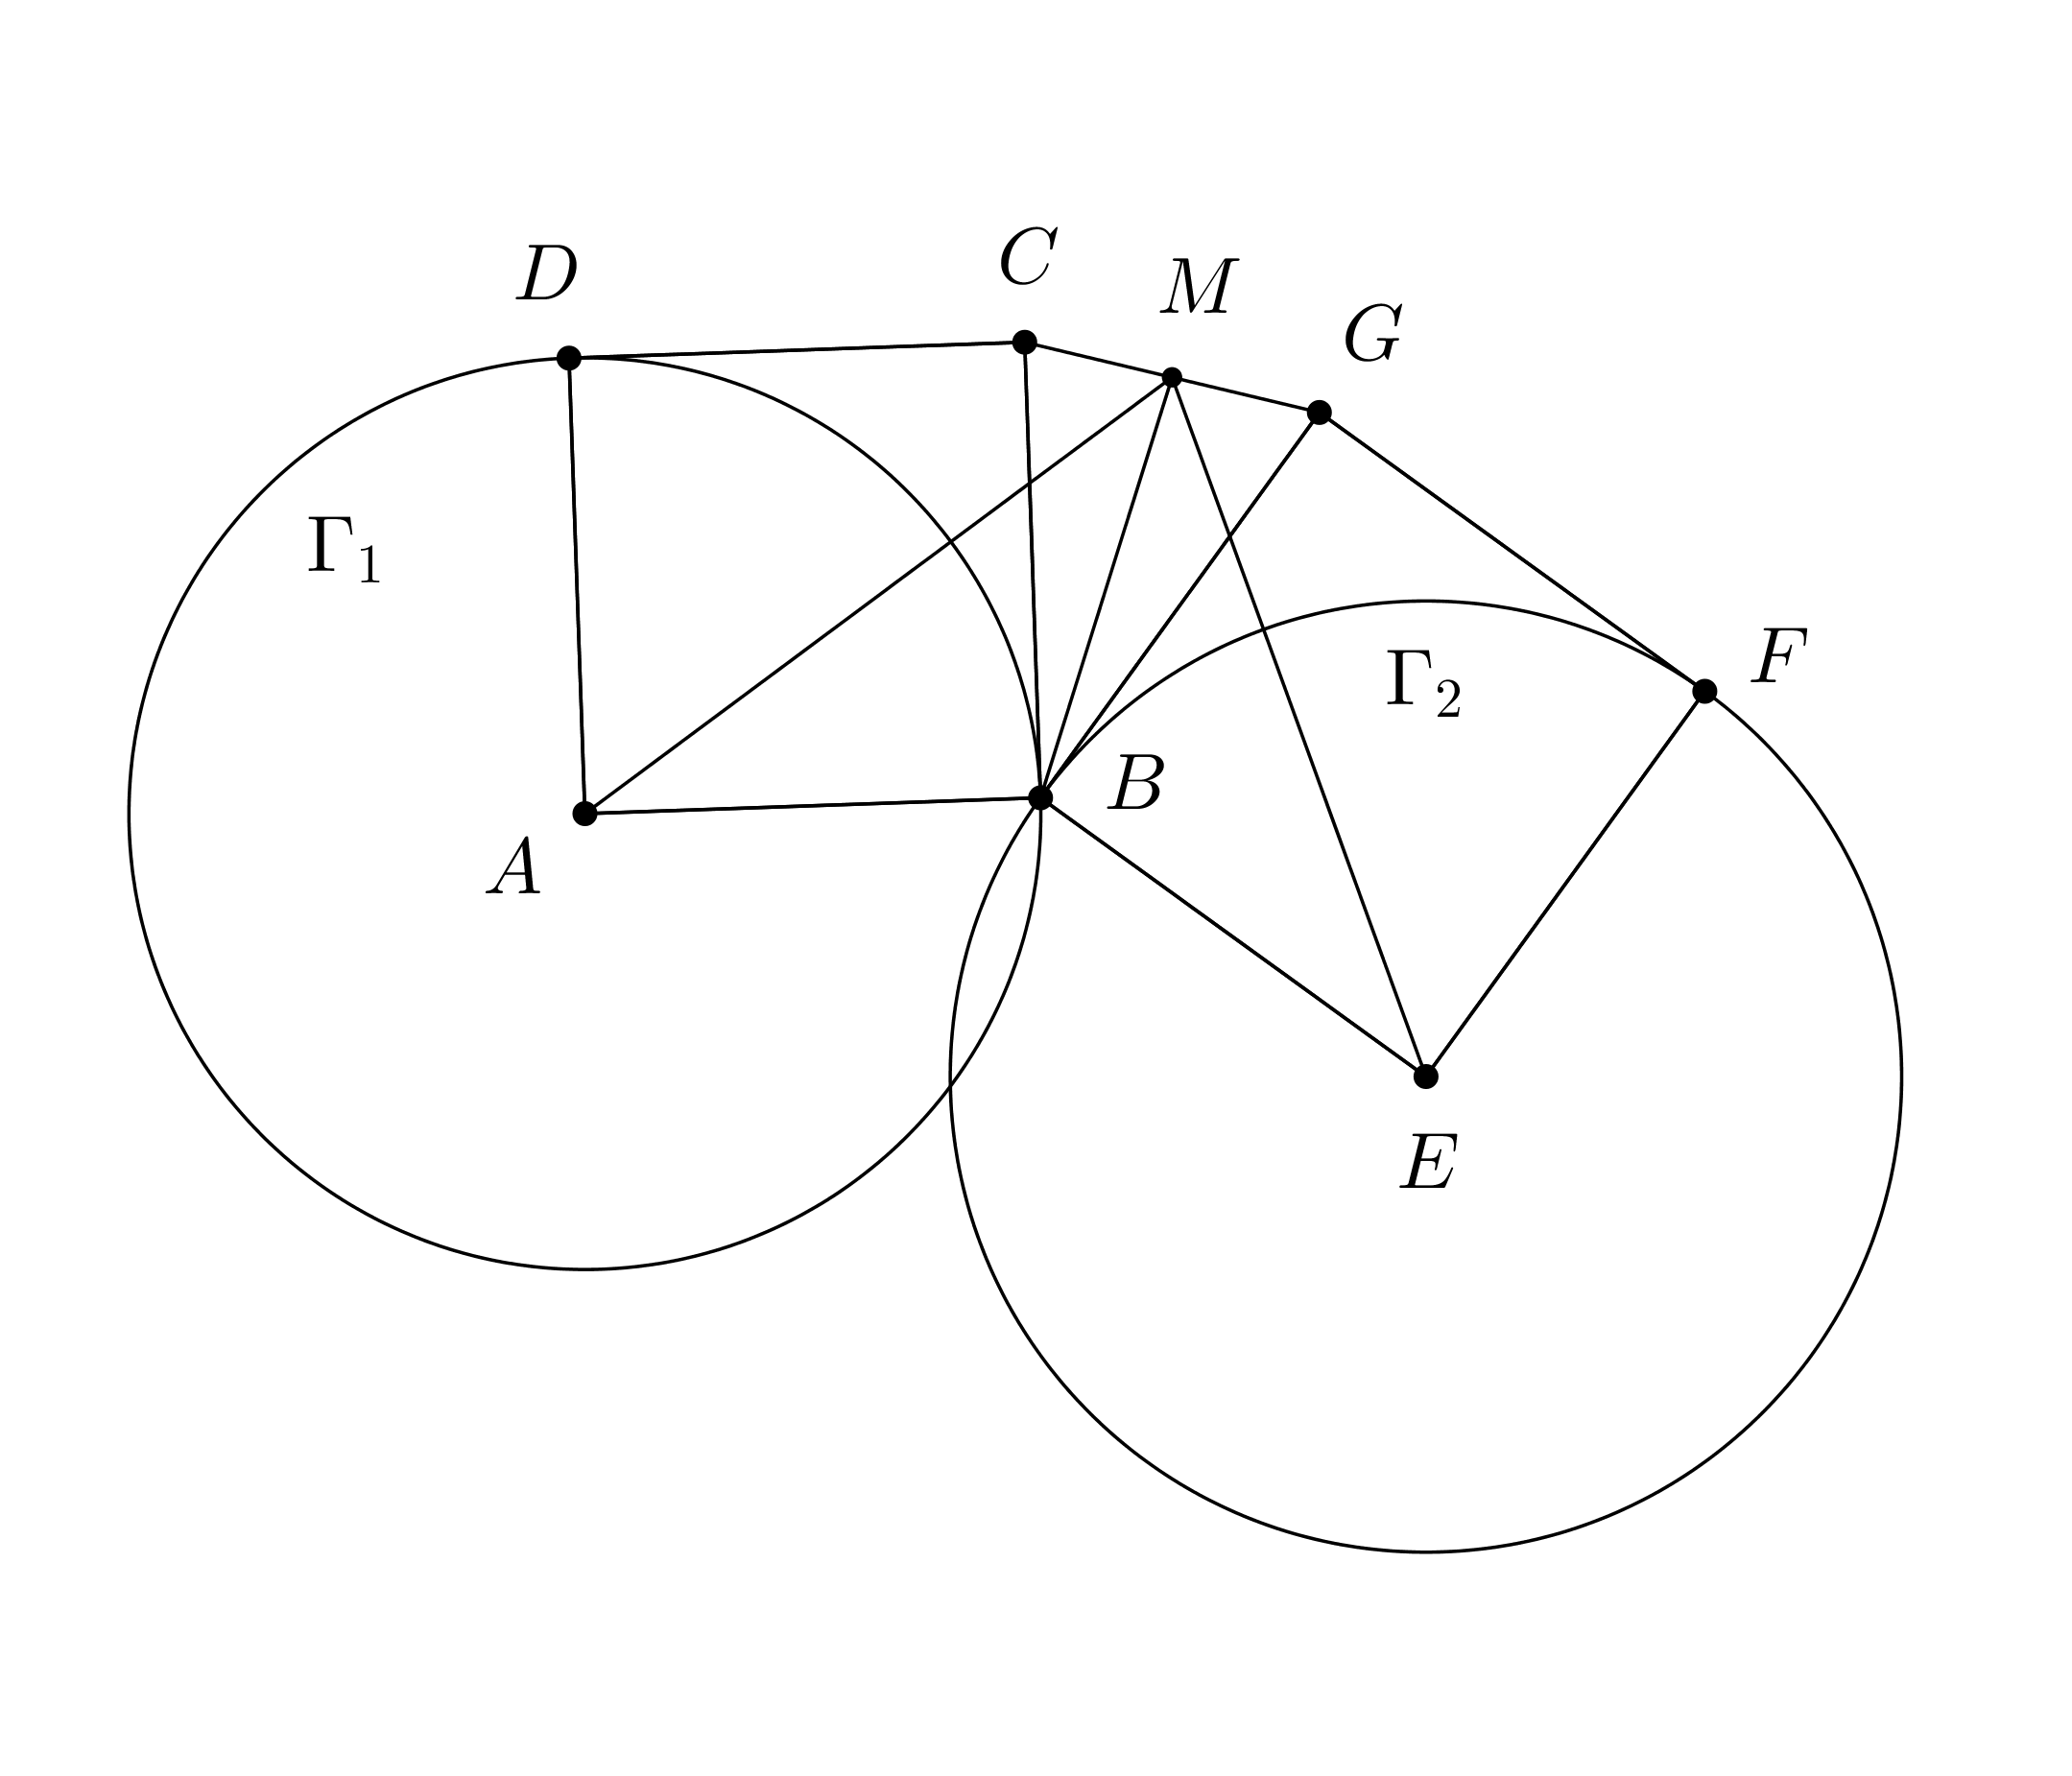
\includegraphics[width=0.8\textwidth]{march_q2.png}
\caption{Problem 2}
\end{figure}

\item % PP-2006-3
%A hexagon can be partitioned into triangles, each coloured either black or white, such that:
%\begin{enumerate}
%\item Every two triangles either share a common side (and then they are of different colours) or a common vertex, or else they have no points in common.
%\item Every side of the hexagon is also a side of one of the black triangles.
%\end{enumerate}

%\begin{center}
%    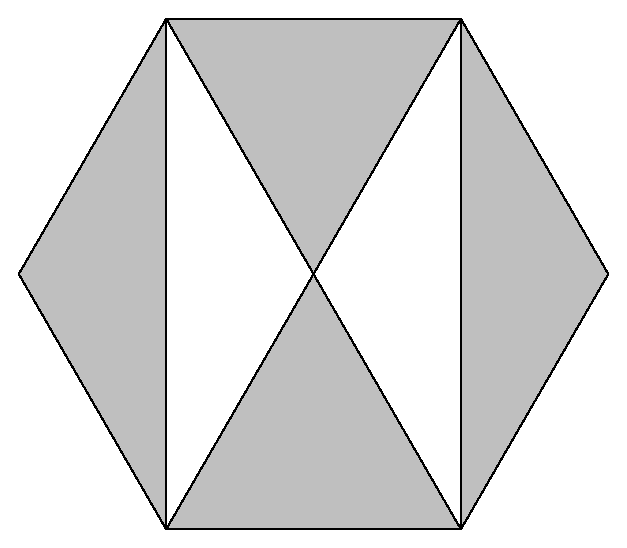
\includegraphics[width=6cm]{march_hexagon.eps}
%\end{center}
%
%Prove that a decagon cannot be partitioned in this way.
Let the number of white triangles be $w$, and the number of black triangles be
$b$. Each edge except for the edges of the decagon is part of exactly one white
triangle, and each white triangle has three edges. It follows that the total
number of edges is $3w + 10$. On the other hand, each edge (including those of
the decagon) is part of exactly one black triangle, and each black triangle has
three edges. Thus the total number of edges is also equal to $3b$. We thus have
that $3w + 10 = 3b$, which is a contradiction since $10$ is not divisible by
$3$.


\item % SW-2013-4
%Determine all pairs of functions $(f,g)$ from the set of real numbers to itself such that
%\[ \min(f(x),f(y)) = \max(g(x),g(y)) \]
%for all real numbers $x$ and $y$ with $x \neq y$.
We claim that $f$ is bounded below. Suppose not. Then there is some $x$ such
that $f(x) < \min\{f(0), g(0) \}$. Since $f(x) < f(0)$, we have that $x \neq 0$,
and so
\[
    f(x) = \min\{ f(x), f(0) \} = \max\{ g(x), g(0) \} \geq g(0),
\]
a contradiction. Let $c$ be the greatest lower bound of the values of $f$.

A similar argument shows that $g$ is bounded above. Let $d$ be the least upper
bound of the values of $g$. We will show that $c = d$.

For any $x \neq y$, we have that
\[
    c \leq \min\{ f(x), f(y) \} = \max\{ g(x), g(y) \} \leq d.   
\]

Thus $c \leq d$. Suppose that $c < d$. Since $c$ is the greatest lower bound of
the values of $f$, we have that $d$ is not a lower bound, and so there is some
$x$ such that $c \leq f(x) < d$. Similarly, since $f(x)$ is not an upper bound
for the values of $g$, there is some $y$ such that $f(x) < g(y) \leq d$. If $y
\neq x$, then we have that
\[
    f(x) \geq \min\{ f(x), f(y) \} = \max\{ g(x), g(y) \} \geq g(y) > f(x),
\]
a contradiction. Otherwise, we have $y = x$, and so for any $z \neq x$, we have
that
\[
    f(x) \geq \min\{ f(x), f(z) \} = \max\{ g(x), g(z) \} \geq g(x) > f(x),
\]
which is again a contradiction. Thus we have that $c = d$.

Now suppose that $x \neq y$ are such that $f(x) > c$ and $f(y) > c$. The we have
that
\[
    c < \min\{ f(x), f(y) \} = \max\{ g(x), g(y) \} \leq d = c,
\]
a contradiction. It follows that there is at most one value of $x$ such that
$f(x) > c$. Similarly, there is at most one value of $y$ such that $g(y) < c$.
All solutions are thus of the form $(f, g)$ where
\[
    f(x) = \begin{cases} c_0 & \text{if } x \neq d_0 \\
        c_1 & \text{if } x = d_0
    \end{cases}
    \quad \text{and} \quad
    g(x) = \begin{cases} c_0 & \text{if } x \neq d_1 \\
        c_2 & \text{if } x = d_1
    \end{cases}
\]
for some constants $c_0, c_1, c_2, d_0$ and $d_1$ such that $c_1 \geq c_0$ and
$c_2 \leq c_0$.

We now check that all such pairs of functions do satisfy the conditions in the
problem. Suppose that $f$ and $g$ are as defined above. Consider any real
numbers $x \neq y$. Since $x \neq y$, we can not have that $x = y = d_0$, and so
either $f(x) = c_0$ or $f(y) = c_0$. Since $c_0 \leq c_1$, this implies that
$\min\{ f(x), f(y) \} = c_0$.

Similarly, we have that $\max\{ g(x), g(y) \} = c_0$. We thus have that
\[
    \min\{ f(x), f(y) \} = c_0 = \max\{ g(x), g(y) \},
\]
as required.

\item % Argentine National Olympiad 2016 1st Level Q2 -- C, Q4
%Given 100 infinitely large boxes with finitely many markers in each of them, the following procedure is carried out: At step 1 one adds one marker in every box. At step 2 one marker is added in every box containing an even number of markers. At step 3 one marker is added in every box in which the number of markers is divisible by 3, and so on. Before the process starts Bruno wants to distribute several markers in the boxes such that there is at least one marker in each box and the following holds: after any number of steps there exist two boxes containing a different number of markers. Is it possible for Bruno to do this?
Consider an arbitrary box, and let $f(n)$ be the number of markers in the box at
the start of the $n^\text{th}$ step. (Before a marker is potentially added on
that step.) Since we never remove a marker from the box, $f$ is non-decreasing.

We claim that $f(n) \geq n$ for all $n$. This is true for $n = 1$ since there is
initially at least one marker in each box. Suppose that $f(n) \geq n$ for some
$n$. If $f(n) = n$, then we add a marker to the box on the $n^\text{th}$ step,
and so $f(n + 1) = n + 1$. Otherwise, we have that $f(n + 1) \geq f(n) \geq n +
1$. The claim follows by induction. It follows that $f(n)$ is unbounded.

Let $p$ be a prime number larger than $f(1)$. Since $f(n)$ is unbounded, and $f$
increases by at most $1$ on each step, there is some $m$ such that $f(m) = p$.
Since $p$ is not divisible by any of the numbers $m, m + 1, \dots, p - 1$, we
see that we do not add any markers to the box until the $p^\text{th}$ step, and
so $f(m) = f(m + 1) = \dots = f(p) = p$. It is then easy to see that $f(n) = n$
for all $n \geq p$.

For each of the 100 boxes, we thus have that eventually the number of markers
in the box is equal to the number of the step that we are on. It follows that,
regardless of the initial distribution of the markers, there will
eventually be the same number of markers in each box, and so Bruno can not
achieve his goal.

\item % SW-2009-6
%Let $n > 1$ be an integer. Prove that the inequality
%\[ \frac{(n-1)^2}{4} \geq \left(\sum_{1 \leq i < j \leq n} \sqrt{x_i x_j}\right)^2 + \left(\sum_{1 \leq i < j \leq n} \left\lvert x_i-x_j \right\rvert \right)^2 \]
%holds for all nonnegative real numbers $x_1, x_2, \dotsc, x_n$ with $x_1 +x_2 +\dotsb +x_n = 1$.
We have that
\begin{align*}
    (n - 1)^2 & - 4 \left(\sum_{1 \leq i < j \leq n} \sqrt{x_i x_j} \right)^2 
     = \left( (n - 1) \sum_{1 \leq i \leq n} x_i \right)^2 - 4 \left(\sum_{1
    \leq i < j \leq n} \sqrt{x_i x_j} \right)^2 \\
    & = \left( (n - 1) \sum_{1 \leq i \leq n} x_i - 2 \sum_{1 \leq i < j \leq n}
    \sqrt{x_i x_j} \right) \left( \ (n - 1) \sum_{1 \leq i \leq n} x_i + 2
    \sum_{1 \leq i < j \leq n} \sqrt{x_i x_j} \right) \\
    & = \left( \sum_{1 \leq i < j \leq n} (\sqrt{x_i} - \sqrt{x_j})^2 \right)
        \left( \sum_{1 \leq i < j \leq n} (\sqrt{x_i} + \sqrt{x_j})^2 \right).
\end{align*}

By the Cauchy-Schwarz inequality, this is greater than or equal to
\[
    \left( \sum_{1 \leq i < j \leq n} | \sqrt{x_i} - \sqrt{x_j} | | \sqrt{x_i} +
    \sqrt{x_j} | \right)^2 = \left( \sum_{1 \leq i < j \leq n} | x_i - x_j |
    \right)^2,
\]
and thus we have that
\[
    \frac{(n - 1)^2}{4} \geq \left( \sum_{1 \leq i < j \leq n} \sqrt{x_i x_j}
    \right)^2 + \frac{1}{4} \left( \sum_{1 \leq i < j \leq n} |x_i - x_j|
    \right)^2,
\]
as desired.

\item % Hard (Med-Hard?) Dutch BxMO Selection Test 2016
%$\triangle ABC$ is right-angled with $\angle A=90^\circ$ and circumcircle $\Gamma$. The incircle of $\triangle ABC$ touches $BC$ at $D$, $CA$ at $E$ and $AB$ at $F$. Let $M$ be the midpoint of arc $AB$ of $\Gamma$ not containing $C$ and let $N$ be the midpoint of arc $AC$ of $\Gamma$ not containing $B$. Prove that $E$, $F$, $M$ and $N$ lie on a straight line.
Let $I$ be the incentre of $\triangle ABC$. Note that $M$ is the intersection of
$CI$ with $\Gamma$, and $N$ is the intersection of $BI$ with $\Gamma$. Since
$BC$ is a diameter of $\Gamma$, we have that $\angle INC = \angle BNC = \angle
BMC = \angle BMI = 90^\circ$. Radii are perpendicular to tangents, and so we
have that $\angle IEC = \angle BFI = 90^\circ$. We see that $IENC$ and $BMFI$
are cyclic. It follows that $\angle ENB = \angle ENI = \angle ECI = \angle ICB =
\angle MCB = \angle MNB$, and so $E$ lies on $MN$. Similarly, we have that
$\angle CMF = \angle IMF = \angle IBF = \angle CBI = \angle CBN = \angle CMN$,
and so $F$ also lies on $MN$.

\begin{figure}[!ht]
\centering
\includegraphics[width=0.8\textwidth]{march_q7.png}
\caption{Problem 7}
\end{figure}

\item % JM-2007-4
%Let $m,n$ be positive integers and $p > 3$ a prime number such that $\gcd(m,p-1) = \gcd(n,p-1) = 1$, and assume that $(a^m + b^m)^n \equiv (a^n + b^n)^m \pmod{p}$ for all integers $a$ and $b$.
%
%Prove that $m \equiv n \pmod{p-1}$.


\end{enumerate}

\end{document}
